\documentclass{article}
\usepackage{fancyhdr} % Required for custom headers
\usepackage{lastpage} % Required to determine the last page for the footer
\usepackage{extramarks} % Required for headers and footers
\usepackage{graphicx} % Required to insert images
%\usepackage{lipsum} % Used for inserting dummy 'Lorem ipsum' text into the template
\usepackage{amsmath}
%\usepackage{amsfont}
%\usepackage{amssymb}

\usepackage{multicol}
% Margins
\topmargin=-0.5in
\evensidemargin=0in
\oddsidemargin=-0.5in
\textwidth=7.5in
\textheight=9.0in
\headsep=0.25in 


\pagestyle{fancy}

\rhead{Elise Bauer} % Top right header
\lhead{Mashed Potatoes}
\chead{ }
%\title{}

\begin{document}
%
%PRELIMINARIES:
%
%
%Begin by preheating the oven to 350 $^o$F
%
%\bigskip
%
%\bigskip

\begin{multicols}{2}
Ingredients:
\begin{itemize}
\item 2 potatoes, peeled and cut lengthwise into quarters
\item 1/2 teaspoon salt
\item 2 Tbsp (30 g) butter
\item 1 Tbsp milk (or more)
\item Salt and Pepper
\end{itemize}
\columnbreak

Directions:
\begin{enumerate}
\item Place the peeled and cut potatoes into a medium saucepan. 
\item Add cold water to the pan until the potatoes are covered by at least an inch. 
\item Add a half teaspoon of salt to the water.
\item Turn the heat on to high, and bring the water to a boil. 
\item Reduce the heat to low to maintain a simmer, and cover. 
\item Cook for 15 to 20 minutes, or until you can easily poke through them with a fork.
\item While the potatoes are cooking, melt the butter and warm the cream. You can heat them together in a pan on the stove or in the microwave.
\item When the potatoes are done, drain the water and place the steaming hot potatoes into a large bowl. Pour the heated cream and melted butter over the potatoes.
\item Mash the potatoes with a potato masher. Then use a strong wooden spoon (a metal spoon might bend) to beat further.
\item Add milk and beat until the mashed potatoes are smooth. Don't over-beat the potatoes or the mashed potatoes will end up gluey.
\item Add salt and pepper to taste.
\end{enumerate}




\end{multicols}



\begin{center}
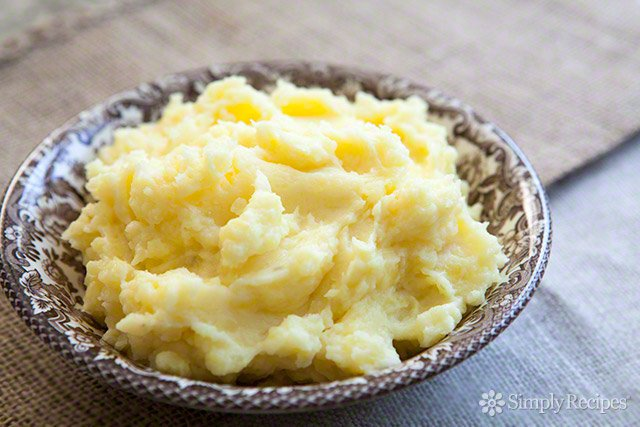
\includegraphics[scale=0.4]{mashedPotatoes.jpg}
\end{center}


\end{document} 











